% !TEX ROOT=./main.tex



\section{Numerical Experiments}



\subsection{Strongly Convex}

\begin{figure}[h!]
\centering
\begin{tabular}{cc}
	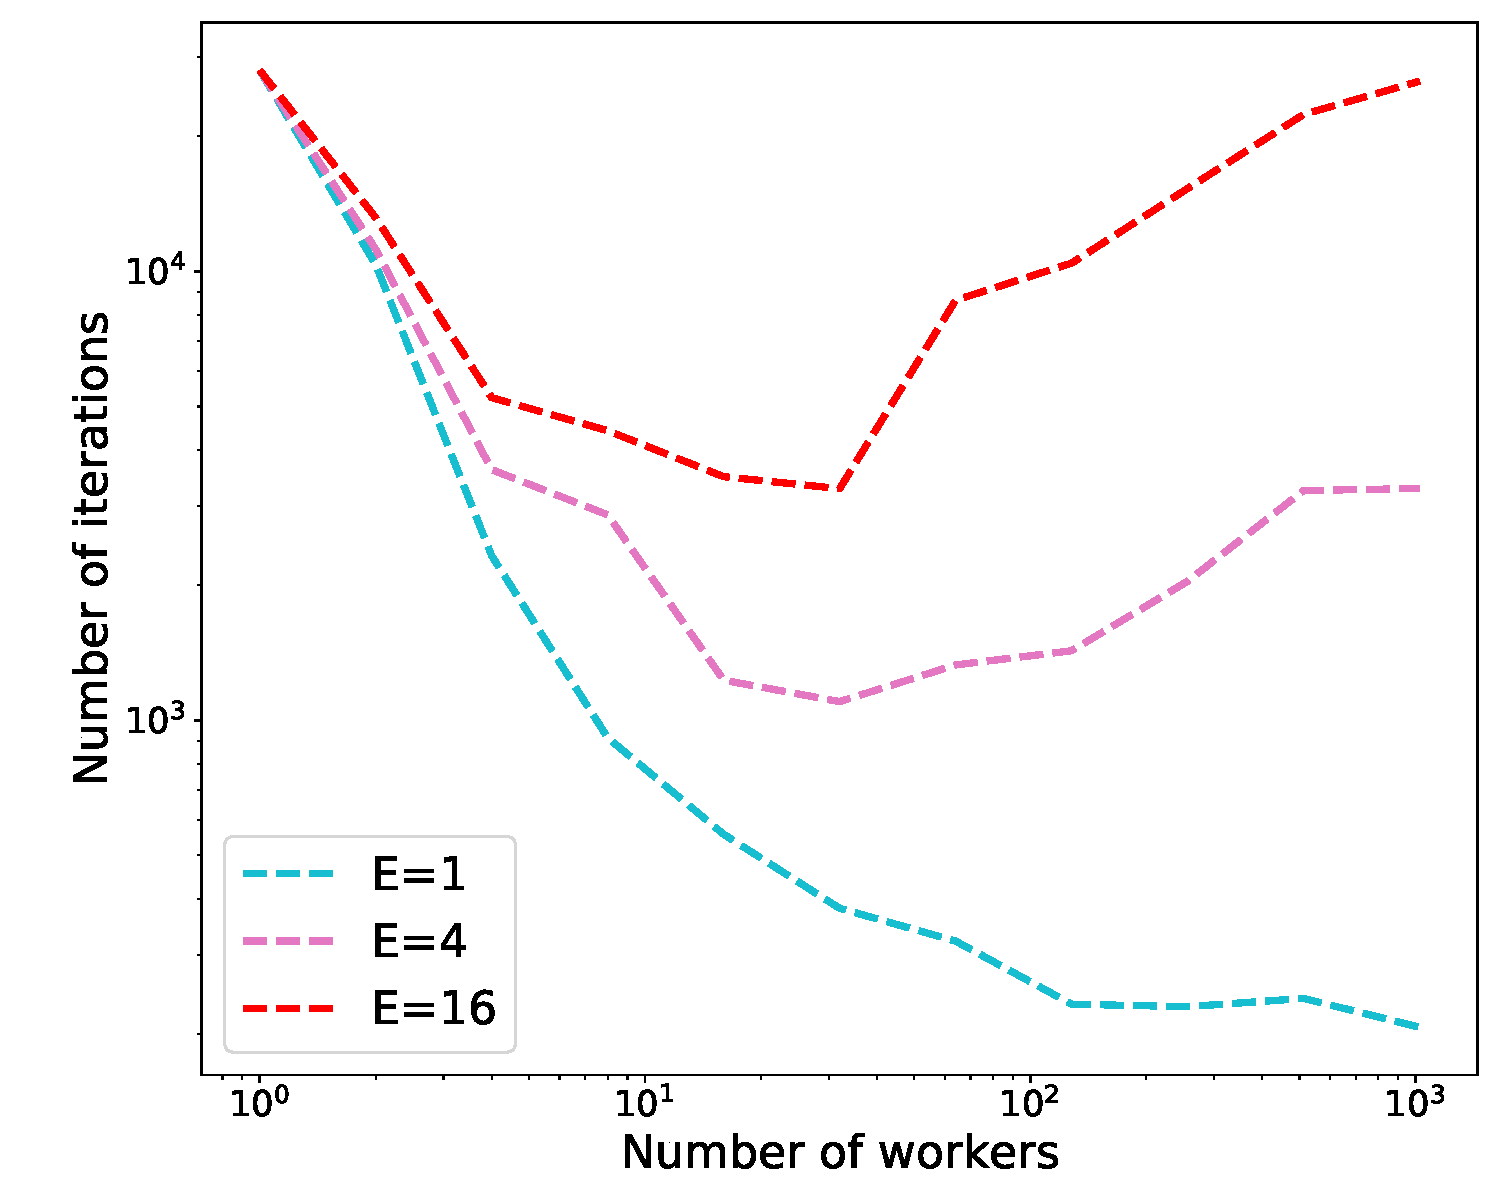
\includegraphics[width=0.5\textwidth]{fig/E1-4-16speedupNodesT-min-w8a-epsilon013-b4-reg1e-05-adapt0.pdf} & 
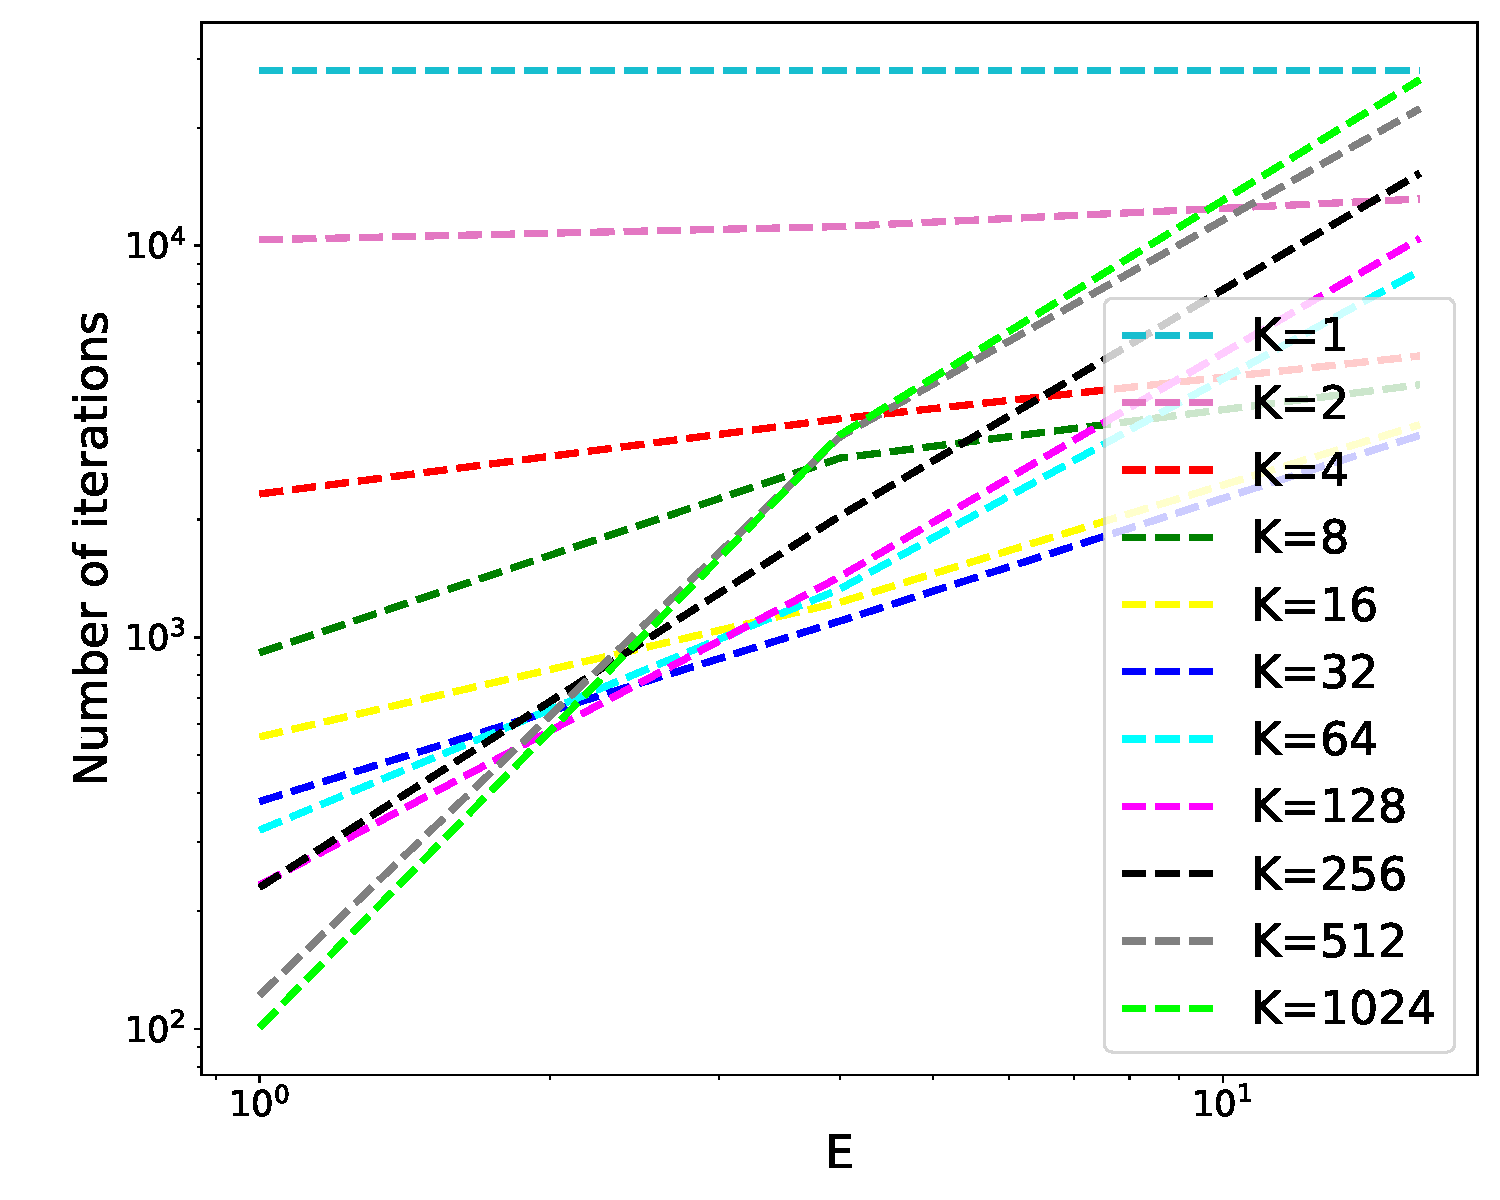
\includegraphics[width=0.5\textwidth]{fig/E1-4-16speedupEpochsT-min-w8a-epsilon013-b4-reg1e-05-adapt0.pdf} \\
	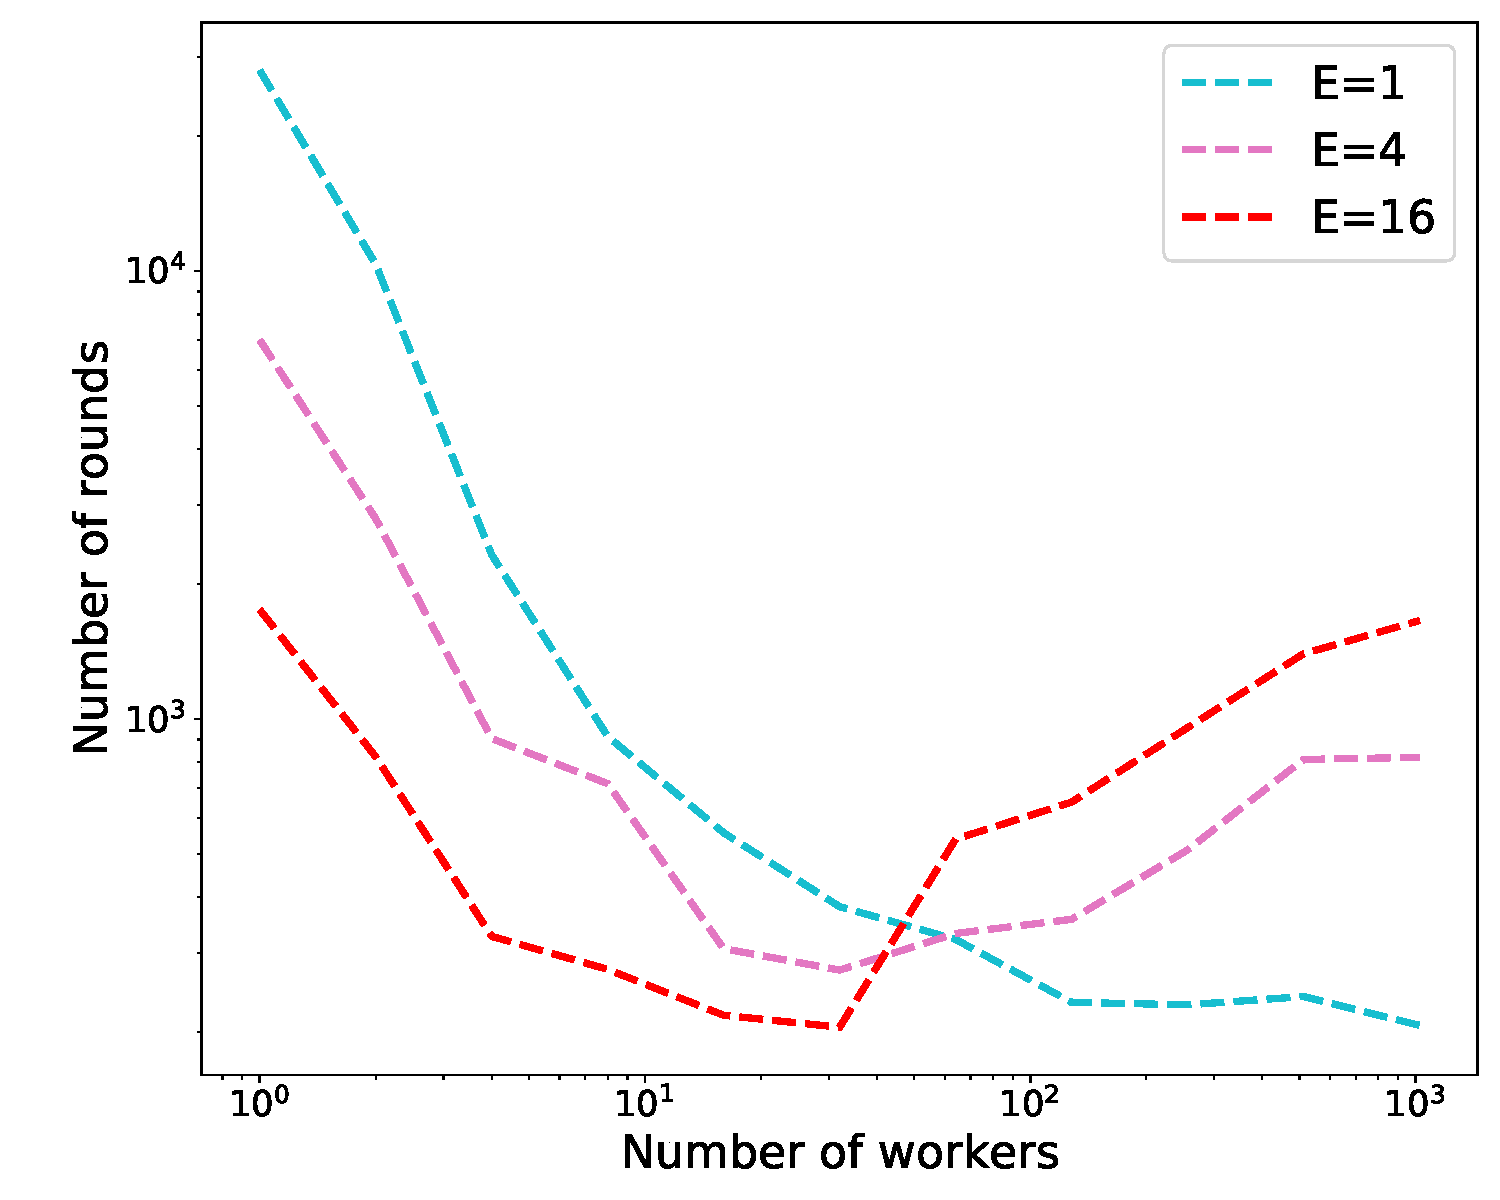
\includegraphics[width=0.5\textwidth]{fig/E1-4-16speedupNodesRounds-w8a-epsilon013-b4-reg1e-05-adapt0.pdf} & 
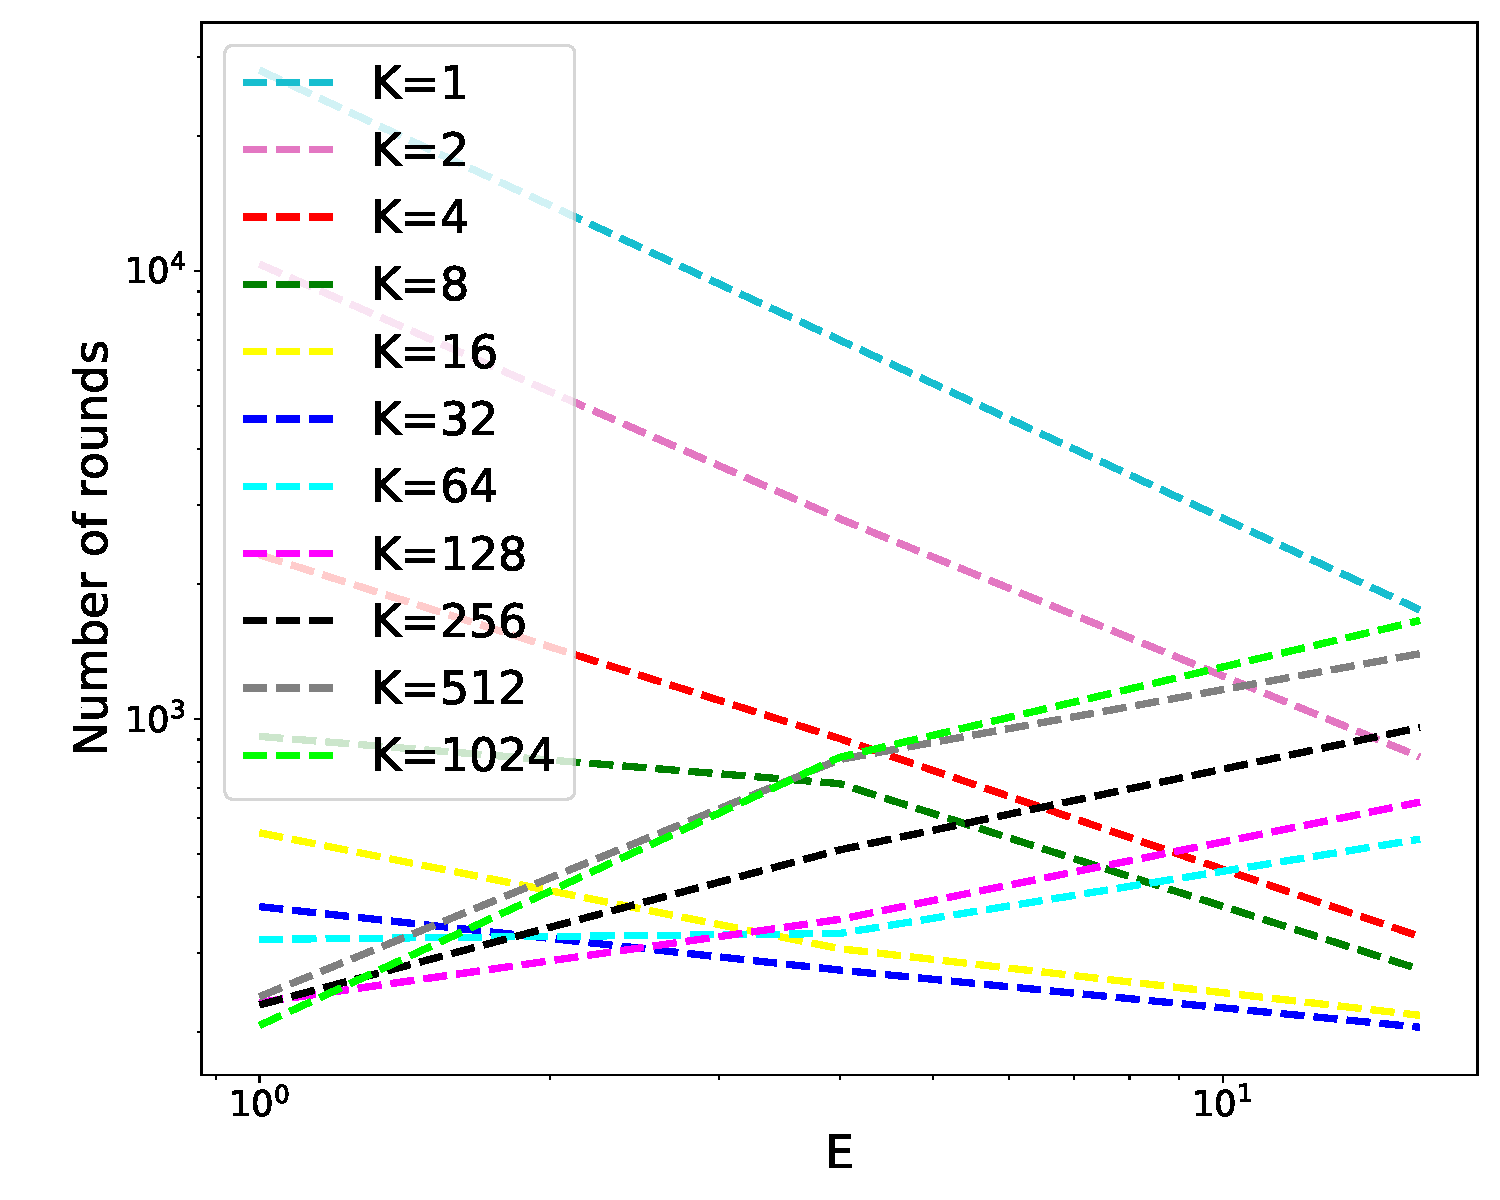
\includegraphics[width=0.5\textwidth]{fig/E1-4-16speedupEpochsRounds-w8a-epsilon013-b4-reg1e-05-adapt0.pdf} \\
\end{tabular}
	\caption{Logistic regression with regularization $1e-5$. The linear speed up w.r.t the number of nodes and number of epochs. The synthetic dataset has $N=49749$ samples, evenly distributed on $1, 2, 4, 8, 16, 32, 64, 128, 256, 512, 1024$ devices. The figure shows the number of iterations/rounds needed to converge to $\epsilon-$accuracy. The learning rate is decayed as the $\eta_t = \min(32, \frac{Nc}{1 + t})$, where we extensively search the best learning rate $c \in \{2^{-1}c, 2^{-2}c, c, 2c, 2^{2}c\}$ and for each configuration. Batch size is 4 in this case.}
\end{figure}



\subsection{Convex smooth objective}






\subsection{Linear regression}





